\begin{boxE}
 \lr{
 \lstinputlisting[language=Python]{IR5/code/job_1.py}
 }   
\end{boxE}

\begin{figure}
    \centering
    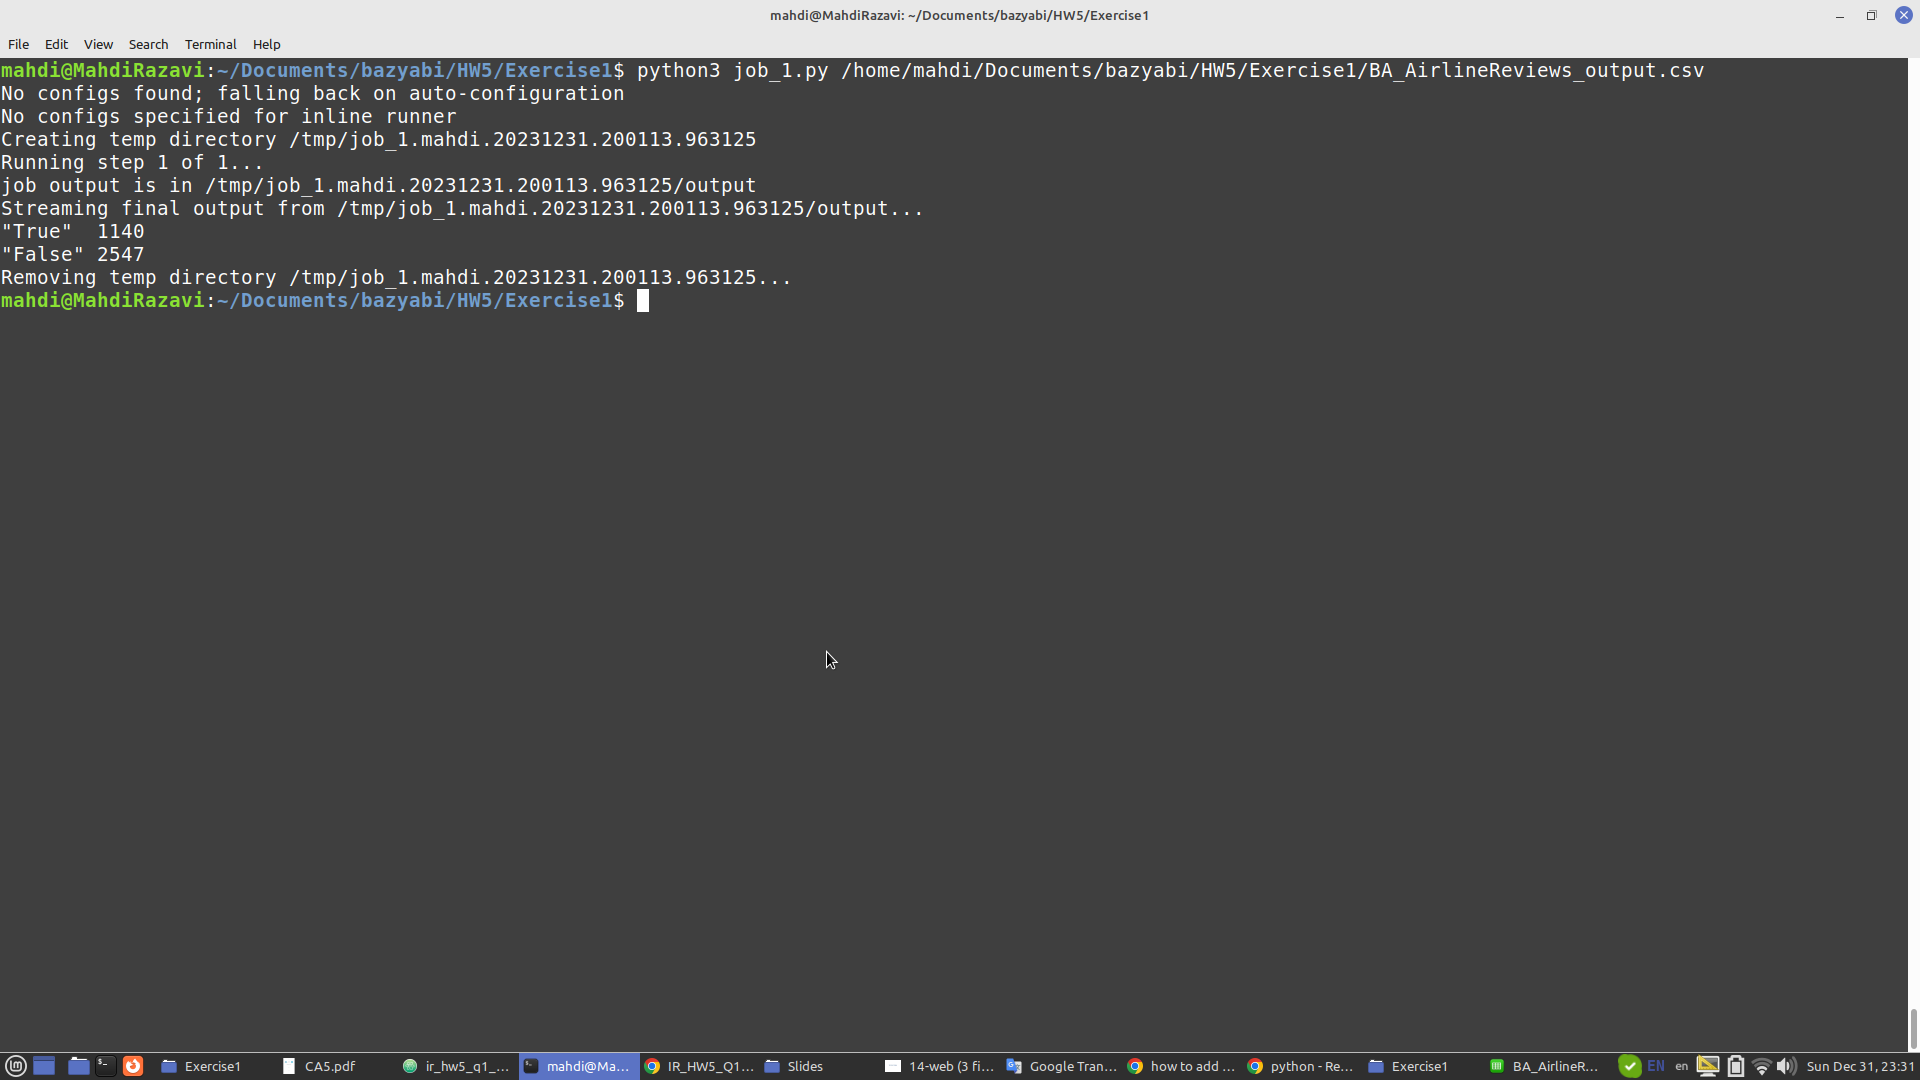
\includegraphics
    [width = 0.9\textwidth]
    {IR5/image/MapReduce1.png}
    \caption{نتایج حاصل از اجرای کد برای شمارش میزان نظرات تایید شده و تایید نشده}
    \label{fig:enter-label}
\end{figure}

\begin{boxM}
    % توضیحات نوشته شود
    در این تمرین در قسمت 
    \lr{Mapper}
    در هر سطر هر یک از دو مقدار 
    \lr{Boolean}
    اتفاق‌افتاده در آن سطر و ستون مدنظر
    را به عدد یک نظیر می‌کنیم.

    سپس در گام 
    \lr{Reducer}
    میزان جمع هر کدام از این مقادیر
    \lr{Boolean}
    را محاسبه خواهیم‌کرد.
    در واقع این گام یک 
    \lr{Aggregator}
    برای ما خواهد بود.   
    تابع 
    \lr{Aggregator}
    ما 
    \lr{Sum}
    خواهد بود.
    
\end{boxM}